\section{Pillar 3: Language as Learning Signal}%
\label{sec:pillar3}
The method above leave the model unchanged; we now examine how verbal feedback can persistently reshape the policy through training. As illustrated in Figure~\ref{fig:training_time}, the four subcategories form a compression spectrum: from feedback-conditioned modeling (\S\ref{sec:feedback-conditioned}), which preserves full critiques, through self-improvement (\S\ref{sec:self-improvement}) and process supervision (\S\ref{sec:process-supervision}), to preference shaping (\S\ref{sec:preference-shaping}), which reduces verbal judgement to a single scalar.

% This pillar covers methods where verbal feedback produces persistent model improvement rather than transient inference-time refinement: language is converted into training signals that update the policy itself. As illustrated in Figure~\ref{fig:training_time}, the four subcategories form a compression spectrum: from feedback-conditioned modeling (\S\ref{sec:feedback-conditioned}), which preserves full natural-language critiques during training, through self-improvement (\S\ref{sec:self-improvement}) and process supervision (\S\ref{sec:process-supervision}), which progressively filter and compress language, to preference shaping (\S\ref{sec:preference-shaping}), which reduces verbal judgement to a single scalar. 
% The compression level also determines the optimization method: methods preserving language train via supervised fine-tuning on filtered or conditioned text, while methods compressing to scalars optimize via RL objectives such as PPO or DPO.
% This spectrum captures a fundamental tradeoff: richer linguistic signals retain more information but are harder to optimize, while scalar compression enables standard gradient-based updates at the cost of discarding feedback structure.


% Pillar 2 focuses on methods where verbal feedback produces persistent model improvement rather than transient inference-time refinement. Instead of guiding a single trajectory, language is converted into training signals that update the policy itself. We organize this pillar by how language enters the training process. In Feedback-Conditioned Modeling (\S\ref{sec:feedback-conditioned}), critiques remain in natural language and are directly conditioned upon during training. In Self-Improvement (\S\ref{sec:self-improvement}), model-generated outputs become training data. In Process Supervision (\S\ref{sec:process-supervision}), intermediate reasoning steps are individually verified. In Preference Shaping (\S\ref{sec:preference-shaping}), verbal judgments are compressed into scalar preferences. 

\subsection{Feedback-Conditioned Modeling}%
\label{sec:feedback-conditioned}



At the upper end of the compression spectrum, feedback-conditioned modeling maintains verbal critiques in their entirety by conditioning the model directly on natural-language feedback during training. The training signal consists of a triple $(x, v, a^*)$: the input, a critique of an initial response, and the revised output. A central question is whether to retain the critique within the training context. Early studies omitted the critique, using only the refined output as the supervision target \citep{scheurer2023training}. Subsequent work, such as ALT \citep{lloret2024towards}, demonstrated that retaining feedback as conditioning context enables models to learn explicit mappings from critique to correction. \citet{luo2025fcp} further formalized this approach by treating free-form feedback as a primary conditioning signal with online bootstrapping. While preserving the full linguistic content of the critique allows these methods to retain the richest signal, this same receptiveness introduces a risk: models may learn to follow critiques indiscriminately, even when they are incorrect \citep{sharma2024towards}.

 



\subsection{Self-Improvement}
\label{sec:self-improvement}
Self-improvement approaches treat language as filtered text rather than as a conditioning context. The central mechanism is generate-then-filter: the model generates multiple candidate trajectories, verbal feedback signals determine which candidates are retained, and these selected outputs become supervised fine-tuning data for subsequent iterations \citep{singh2023beyond}. The filtering criterion directly shapes the model's learning. For example, in STaR \citep{zelikman2022star}, correctness of the final answer is used as the filter, while in Constitutional AI \citep{bai2022constitutional}, adherence to safety principles serves this role. Explicit labeling is not always required; majority voting across diverse samples can identify likely correct traces \citep{huang2022selfimprove}, and the model itself can act as a judge across iterations \citep{yuan2024self}. This self-contained loop can facilitate compounding improvements over multiple cycles. However, filter quality remains a critical bottleneck: when the same model functions as both generator and judge, systematic biases may be amplified \citep{shumailov2023curse}.




\begin{figure}[t]
     \centering    
    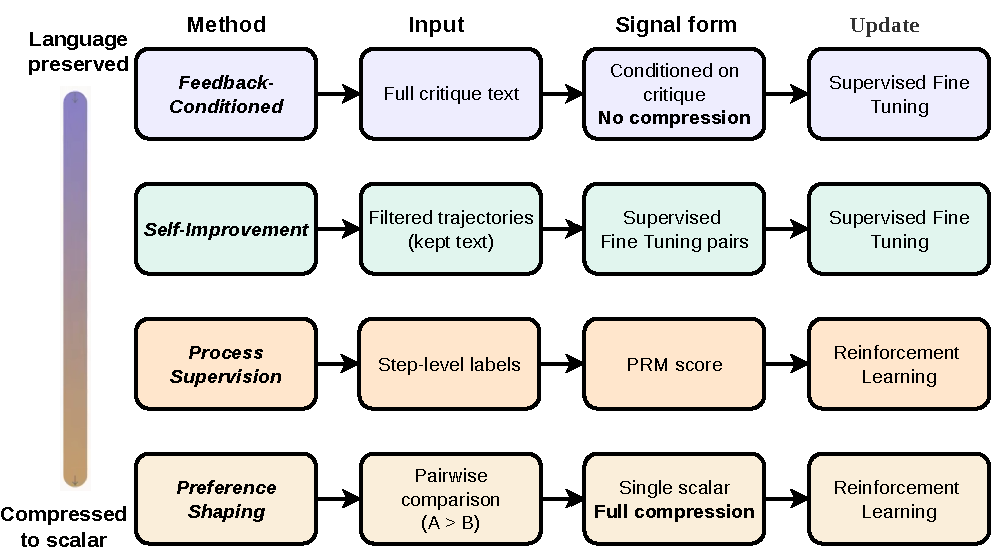
\includegraphics[width=\linewidth]{paper_images/training.pdf}
    \caption{\footnotesize Training-time verbal feedback methods organized by degree of linguistic compression. Methods at the top preserve full natural-language feedback during training, while methods at the bottom compress it into scalar signals.}
    \label{fig:training_time}
\end{figure}

% \das{should we cite some papers on bias of llm as judges ? shumailov I had not read but the name of the paper seems to be somethgn about the data causing the issue, double check}

\subsection{Process Supervision}%
\label{sec:process-supervision}
Process supervision reduces verbal feedback to scalar scores at the step level. Annotators assess each intermediate reasoning step, and these evaluations are used to train a process reward model; the verbal content of the judgments is omitted. Despite this reduction, step-level supervision substantially outperforms outcome-level supervision \citep{lightman2024let, uesato2022solving}, as localized feedback enables more precise credit assignment. The high cost of step-level annotation has motivated efforts to automate this process \citep{wang2024mathshepherdverifyreinforcellms, luo2024improve}. Generative process reward models that incorporate reasoning prior to scoring retain more verbal information while maintaining step-level granularity \citep{zhao2025genprm, liu2025agenticreinforcementlearningimplicit}. Although step-level granularity offers significant advantages, it remains costly and is challenging to define in domains where intermediate correctness is ambiguous.







\subsection{Preference Shaping}%
\label{sec:preference-shaping}


Preference shaping represents the maximal compression of verbal feedback, reducing a comparative judgment between two responses to a single scalar that guides policy updates. Building on the foundation of learning from verbal preferences \citep{christiano2017deep}, InstructGPT \citep{ouyang2022training} demonstrated large-scale implementation by training a reward model on pairwise rankings and optimizing the policy online. Direct Preference Optimization (DPO) \citep{rafailov2023direct} further simplified this process by eliminating the explicit reward model and training directly on preference pairs, using the comparison itself as the loss signal. Subsequent research has investigated additional alternatives \citep{ethayarajh2024kto, hong2024orpo, meng2024simpo, azar2024general}. Notably, \citet{lee2023rlaif} replaced human annotators with AI judges, thereby enhancing the scalability of preference collection. \added{The online and offline variants differ in practice: online optimization against a learned reward model can query feedback on fresh policy samples, while offline objectives such as DPO inherit the coverage of a fixed preference set.} Although scalar compression reduces the explanatory richness of verbal feedback, the scalability enabled by llm generated judgments increasingly justifies this tradeoff. \added{Under our inclusion criteria (Section~\ref{sec:intro}), preference shaping marks the outer boundary of VRL: once the judgment is compressed to a preference bit before any learning, the linguistic structure is no longer consumed, so vanilla RLHF and DPO sit outside the paradigm. We retain them here as the endpoint of the compression spectrum because they clarify, by contrast, what the methods above preserve.}

% Preference shaping converts verbal judgments into scalar optimization signals. Instead of retaining critiques as text, annotators compare candidate outputs and indicate which is preferred. InstructGPT \citep{ouyang2022training} established this paradigm at scale by training reward models on pairwise rankings and optimizing policies with RL. DPO \citep{rafailov2023direct} simplifies the pipeline by optimizing directly on preference pairs without an explicit reward model. Subsequent methods further streamline preference optimization \citep{ethayarajh2024kto, hong2024orpo, meng2024simpo, azar2024general}\das{shouldn't we talk about how they are different? or is this an artifact of Genta's compression? please differentiate them}, while RLAIF \citep{lee2023rlaif} replaces human annotators with AI judges. Preference shaping scales effectively but sacrifices much of the explanatory richness of verbal feedback through scalar compression. \das{we need to make a distinction between online and offline methods, for example DPO vs Online DPO/ RLHF. }






% Process supervision increases feedback granularity from whole outputs to individual reasoning steps. Instead of judging only final answers, annotators verify intermediate steps, producing labels for a process reward model. \citet{lightman2024let} show that step-level supervision substantially outperforms outcome-only supervision, while \citet{uesato2022solving} find it reduces logical reasoning errors more effectively. Later work explores automating step-level annotation \citep{wang2024mathshepherdverifyreinforcellms, luo2024improve}. Although highly effective, process supervision is expensive and currently most practical in domains such as math and code where intermediate correctness is well-defined.
% \das{this section is underspecified. How is standard scalar process reward modeling is verbal reward? you either have to explicitly talk about PRMs that are not scalar rewards or probably consider Generative Reward models, like the one deepseek or something like https://arxiv.org/abs/2509.22638}


% \das{this subsection is perhaps the most appropriate and important in this section, do we want to move this earlier?}
